%!TEX root = ../../Main.tex
\graphicspath{{Chapters/Pol-placering/}}
%-------------------------------------------------------------------------------

\section{Pol-placering}
For at designe en lukket sløjfe controller for ens system, har vi gjort brug af pol-placerings princippet. Dette gøres ved at først at bestemme hvilken orden ens system har (første, anden osv.). Ud fra hvilken orden ens system har kan man lave en karakteristik ligning for denne. I vores tilfælde er det et anden-ordens system, hvilket for ligningen til at se således ud:

\begin{equation}
 \frac{wn^2}{s^2+2*\zeta*wn*s+wn^2}
\end{equation}


Derefter skal vi bestemme nogle krav til systemet. Vi har valgt at vores overshoot skal ligge på 5\% og vores settlingtime til 2 sekunder. Disse krav er forskellige fra system til system og bestemmes af hvad systemet skal bruges til. Når vi har valgt vores settlingtime og overshoot kan vi finde polerne for karakteristikligningen. Disse poler skal bruges til at designe vores controller, så den får den rette karakteristik, altså 5\% overshoot og 2 sekunders settlingtime. Nedenunder kan man se blok opbygningen af et system med state-variable feedback på \autoref{fig:Blok_CL}

\begin{figure}[H]
	\centering
	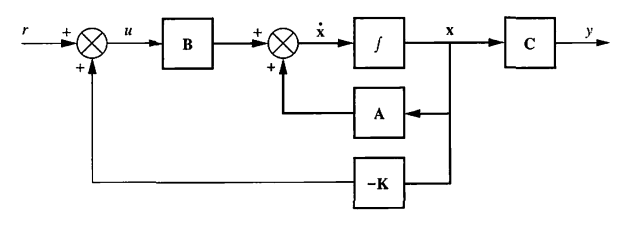
\includegraphics[width = 400pt]{Img/Controller_blok.png}
	\caption{Blok diagram over vores controller}
	\label{fig:Blok_CL}
\end{figure}

Vi gør brug af matlab funktionen place, som kan beregne vores state feedback matrix, K. Dette gør vi ved at indsætte state space variablerne A og B, som vi fandt frem til i starten og polerne fra vores karakteristik ligning. Dermed får vi beregnet vores feedback matrix så den passer med vores krav.
Nu kan vi teste om vores controller fungerer efter hensigten ved at smide et stepinput ind i systemet og kigge på responset. Dette kan ses på \autoref{fig:StepOfSysSS_cl}.  

\begin{figure}[H]
	\centering
	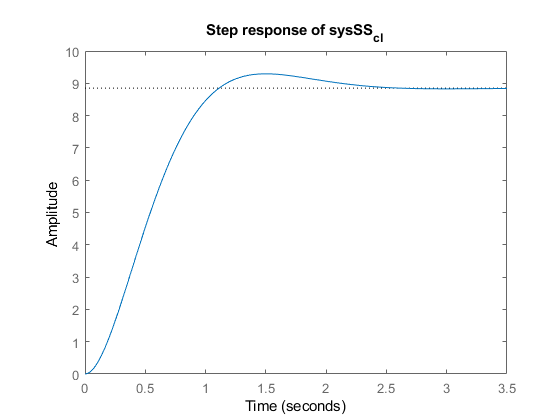
\includegraphics[width = 400pt]{Img/StepOfSysSS_cl.png}
	\caption{Steprespons for closed loop system}
	\label{fig:StepOfSysSS_cl}
\end{figure}

Man kan se systemet har det rette overshoot på 5\% og en settling time på 2 sekunder, dog er der en betydelig steady state fejl da den ender helt oppe i ca 9. Dette betyder at bilen vil køre næsten 9 gange for langt. Dette er ikke optimalt og burde derfor rettes.

\subsection{Steady state error}
Man kan se på step responset på \autoref{fig:StepOfSysSS_cl}, at der er en stor steady state fejl. Man kan se på \autoref{fig:Blok_CL}, at tilbagekoblingen tages fra punktet x, som ligger før C-blokken. Da tilbagekoblingen ikke trækkes fra undgangen y, kommer der højst sandsynligt en form for steady state error.

\begin{figure}[H]
	\centering
	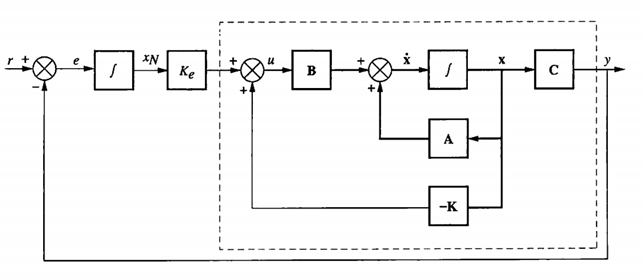
\includegraphics[width = 300pt]{Img/SteadyState_blok.png}
	\caption{Matrix når tredje pol indsættes}
	\label{fig:SteadyState_blok}
\end{figure}

Denne fejl kan elimineres ved at indsætte endnu en pol i systemet. Denne pol skal gerne ligge så langt væk fra de eksisterende poler, at det ikke har nogen indflydelse på systemets karakteristik. Til vores system vælger vi denne tredje pol til at ligge i -30.

På \autoref{fig:SteadyState_blok} kan man se hvordan en ny tilbagekobling introduceres fra punktet y, der derefter trækkes fra referencen r. Derudover er der også kommet en ekstra integrator og gain blok ind i systemet. Det betyder at steady state fejlen lige så stille bliver nul. 

\begin{figure}[H]
	\centering
	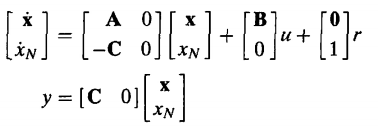
\includegraphics[width = 300pt]{Img/SteadyState_matrix.png}
	\caption{Matrix når tredje pol indsættes}
	\label{fig:SteadyStateMatrix}
\end{figure}

Da vi tilføjer endnu en pol og dermed også gør det til et tredje ordens system, bliver vi nødt til at lave om på vores state space matricer A, B, C og D. De skal udvides så de kommer til at være et tredje ordens system.

Men da inputtet u nu har ændret sig, skal matrixen laves om endnu engang. U er nu:
\begin{equation}
u=-Kx+K_ex_n
\end{equation}
Til sidst indsætter man u ind i matrixen og får den endelige matrix på \autoref{fig:SteadyStateMatrixFinal}

\begin{figure}[H]
	\centering
	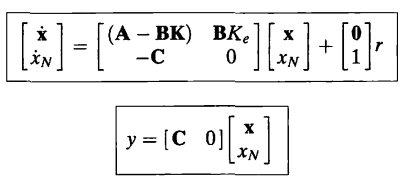
\includegraphics[width = 300pt]{Img/SteadyState_matrix_final.png}
	\caption{Endelig matrix når steady state error skal fjernes}
	\label{fig:SteadyStateMatrixFinal}
\end{figure}

Det har vi så gjort i matlab på følgende måde:

\begin{lstlisting}
%% Insert 3rd pole to eliminate ss error
p3 = -30;
poles_new = [poles' p3];

A_new = [A [0;0];-C 0];
B_new = [B;0];

K_new = place(A_new,B_new,poles_new);
Ke = -K_new(3);
K_new = [K_new(1) K_new(2)];

A_cl_new = [A-B*K_new B*Ke;-C 0];
B_cl_new = [0;0;1];
C_cl_new = [C 0];

sysSS_new = ss(A_cl_new,B_cl_new,C_cl_new,D);

figure
step(sysSS_new);
title('Step response of sysSS_n_e_w with 3rd pole');
\end{lstlisting}

Hvis vi igen tester systemet med et step, kan man se at den stationære fejl nu er 0, og bilen vil altså nu kører præcis så langt, som vi siger den skal køre. Stepresponset kan ses på 

\begin{figure}[H]
	\centering
	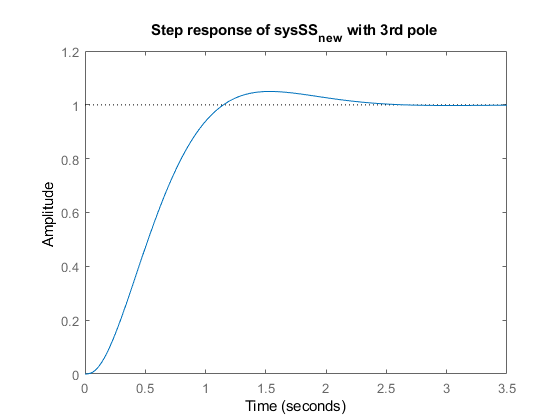
\includegraphics[width = 300pt]{Img/StepOfSySS_new.png}
	\caption{Step respons uden steady state error}
	\label{fig:SteadyState_stepresponse}
\end{figure}